\documentclass[a4paper, 12pt]{report}
\usepackage{cmap}
\usepackage[T2A]{fontenc}
\usepackage[utf8]{inputenc}
\usepackage[english,russian]{babel}
\usepackage{listings}
\usepackage{amsmath}
\usepackage{float}
\usepackage{csquotes}
\usepackage{graphicx}
\graphicspath{ {./images/} }
\usepackage{xcolor}
\definecolor{buzzlightyear}{HTML}{8757A5}
\definecolor{grass}{HTML}{738D06}
\definecolor{literal}{HTML}{F18A2B}
\definecolor{commentcolor}{HTML}{8E908B}

\lstdefinestyle{habrstyle}{
	backgroundcolor=\color{white},
	commentstyle=\color{commentcolor},
	keywordstyle=\bfseries\color{buzzlightyear},
	numberstyle=\tiny\color{commentcolor},
	stringstyle=\color{grass},
	basicstyle=\ttfamily\footnotesize,
	breakatwhitespace=false,         
    	breaklines=true,                 
   	captionpos=b,                    
    	keepspaces=true,                 
    	numbers=left,                    
    	numbersep=7pt,                  
    	showspaces=false,                
    	showstringspaces=false,
   	showtabs=false,                  
    	tabsize=3
}

\lstset{style=habrstyle}

\author{3530901/80201, Шелаев Н. Р.}
\title{Лабораторная работа № 11. Модуляция и выборка (квантование).}
\date{\today}

\begin{document}
	\maketitle
	\tableofcontents
	\listoffigures
	\lstlistoflistings

	\chapter{Свертка с импульсами}
	Свертка с пачкой импульсов - это сложение смещенных и масштабированных копий сигнала.
	\begin{lstlisting}[language=Python,caption=Получение сигнала]
		from thinkdsp import read_wave

		wave = read_wave('253887__themusicalnomad__positive-beeps.wav')
		wave.normalize()
		wave.plot()
	\end{lstlisting}
	\begin{figure}[H]
		\centering
		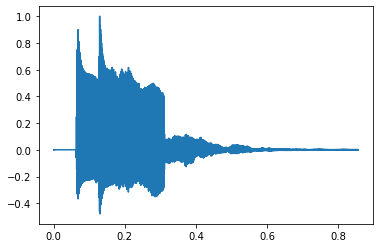
\includegraphics[width=0.75\textwidth]{imp1.png}
		\caption{Полученный сигнал}
		\label{fig:imp1}
	\end{figure}
	\begin{lstlisting}[language=Python,caption=Последовательность из 4-х импульсов]
		from thinkdsp import Impulses

		imp_sig = Impulses([0.005, 0.3, 0.6, 0.9], amps = [1, 0.5, 0.25, 0.1])
		impulses = imp_sig.make_wave(start = 0, duration = 1.0, framerate = wave.framerate)
		impulses.plot()	
	\end{lstlisting}
	\begin{figure}[H]
		\centering
		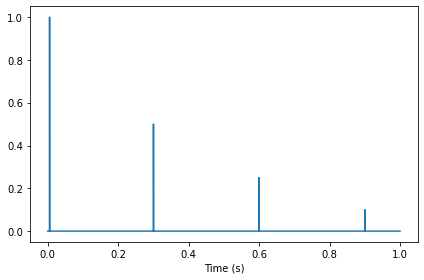
\includegraphics[width=0.75\textwidth]{imp2.png}
		\caption{4 импульса}
		\label{fig:imp2}
	\end{figure}
	\begin{lstlisting}[language=Python,caption=Применим свертку сигнала с импульсами]
		convolved = wave.convolve(impulses)
		convolved.plot()	
	\end{lstlisting}
	\begin{figure}[H]
		\centering
		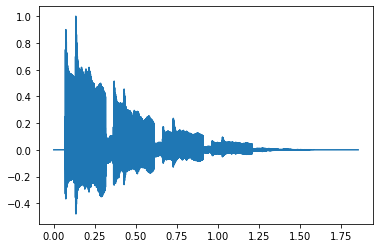
\includegraphics[width=0.75\textwidth]{imp3.png}
		\caption{Результат свертки}
		\label{fig:imp3}
	\end{figure}
	Свертка сигнала с импульсами дает сдвинутые, масштабированные копии сигнала.

	\chapter{Амплитудная модуляция (АМ)}
	АМ - это умножение \textquote{несущего} сигнала с полезным сигналом.
	\begin{lstlisting}[language=Python,caption=Полезный сигнал]
		wave=read_wave('105977__wcfl10__favorite-station.wav')
		wave.unbias()
		wave.normalize()
		spectrum = wave.make_spectrum()
		spectrum.plot()
		spectrum = wave.make_spectrum(full = True)
		spectrum.plot()
	\end{lstlisting}
	\begin{figure}[H]
		\centering
		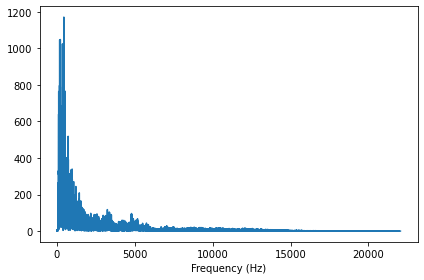
\includegraphics[width=0.75\textwidth]{am1.png}
		\caption{Спектр полезного сигнала}
		\label{fig:am1}
	\end{figure}
	\begin{figure}[H]
		\centering
		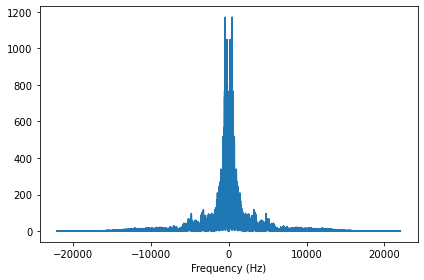
\includegraphics[width=0.75\textwidth]{am2.png}
		\caption{Полный спектр с отрицательными частотами}
		\label{fig:am2}
	\end{figure}
	\begin{lstlisting}[language=Python,caption=Модуляция сигнала косинусоидой]
		from thinkdsp import CosSignal

		carrier_sig = CosSignal(freq = 10000)
		carrier_wave = carrier_sig.make_wave(duration=wave.duration, framerate=wave.framerate)
		modulated = wave * carrier_wave
		modulated.make_spectrum(full = True).plot()
	\end{lstlisting}
	\begin{figure}[H]
		\centering
		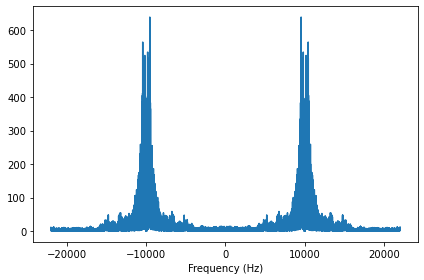
\includegraphics[width=0.75\textwidth]{am3.png}
		\caption{Спектр модулированного сигнала}
		\label{fig:am3}
	\end{figure}
	На слух полученный сигнал не очень приятный, потому что умножение во временной области соответствует свертке в частотной области. АМ имеет эффект разделения спектра на 2 половины и сдвига частот на 10 кГц.
	\begin{lstlisting}[language=Python,caption=Демодуляция сигнала]
		demodulated = modulated * carrier_wave
		demodulated_spectrum = demodulated.make_spectrum(full = True)
		demodulated_spectrum.plot()
		wave.plot()
		demodulated.plot()
	\end{lstlisting}
	\begin{figure}[H]
		\centering
		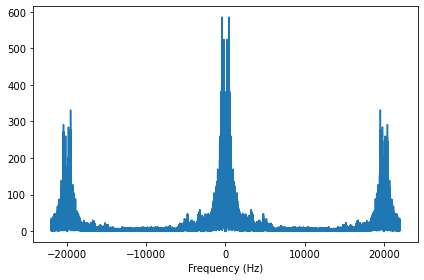
\includegraphics[width=0.75\textwidth]{am4.png}
		\caption{Результат демодуляции сигнала}
		\label{fig:am4}
	\end{figure}
	\begin{figure}[H]
		\centering
		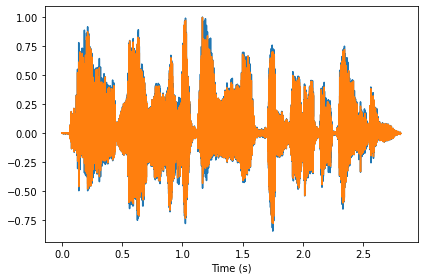
\includegraphics[width=0.75\textwidth]{am5.png}
		\caption{Сравнение исходного и демодулированного сигнала}
		\label{fig:am5}
	\end{figure}
	На слух демодулированный сигнал не отличается от исходного, но на графике видны небольшие различия.
	\begin{lstlisting}[language=Python,caption=Применим ФНЧ]
		demodulated_spectrum.low_pass(10000)
		demodulated_spectrum.plot()
		filtered = demodulated_spectrum.make_wave()
	\end{lstlisting}
	\begin{figure}[H]
		\centering
		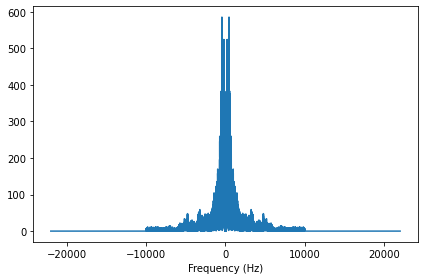
\includegraphics[width=0.75\textwidth]{am6.png}
		\caption{Спектр демодулированного сигнала после применения ФНЧ}
		\label{fig:am6}
	\end{figure}
	\begin{lstlisting}[language=Python,caption=Спектр косинусоиды]
		carrier_spectrum = carrier_wave.make_spectrum(full = True)
		carrier_spectrum.plot()
	\end{lstlisting}
	\begin{figure}[H]
		\centering
		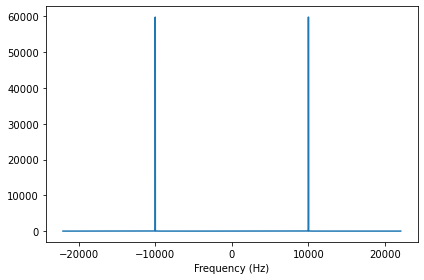
\includegraphics[width=0.75\textwidth]{am7.png}
		\caption{Спектр косинусоиды - два импульса}
		\label{fig:am7}
	\end{figure}
	\begin{lstlisting}[language=Python,caption=Два раза применим свертку сигнала с импульсами]
		convolved = spectrum.convolve(carrier_spectrum)
		convolved.plot()
		reconvolved = convolved.convolve(carrier_spectrum)
		reconvolved.plot()
	\end{lstlisting}
	\begin{figure}[H]
		\centering
		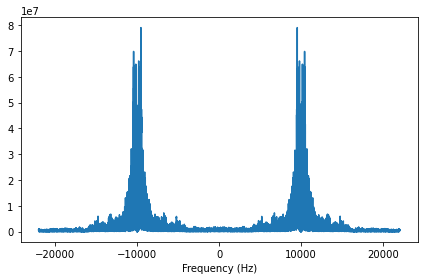
\includegraphics[width=0.75\textwidth]{am8.png}
		\caption{Первая свертка - 2 копии сигнала}
		\label{fig:am8}
	\end{figure}
	\begin{figure}[H]
		\centering
		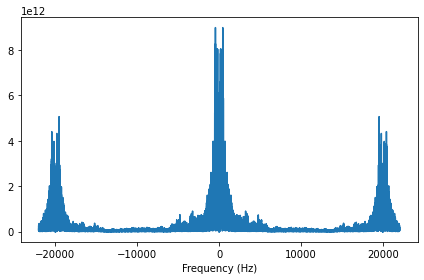
\includegraphics[width=0.75\textwidth]{am9.png}
		\caption{Вторая свертка - 4 копии сигнала}
		\label{fig:am9}
	\end{figure}
	АМ присходит с помощью свертки полезного сигнала с пачкой импульсов \textquote{несущего} сигнала.

	\chapter{Выборка}
	Выборка - процесс измерения аналогового сигнала в серии моментов времени (обычно через равные промежутки).
	\begin{lstlisting}[language=Python,caption=Возьмем интересный сигнал]
		wave = read_wave('263868__kevcio__amen-break-a-160-bpm.wav')
		wave.normalize()
		wave.plot()
		wave.make_spectrum(full = True).plot()
	\end{lstlisting}
	\begin{figure}[H]
		\centering
		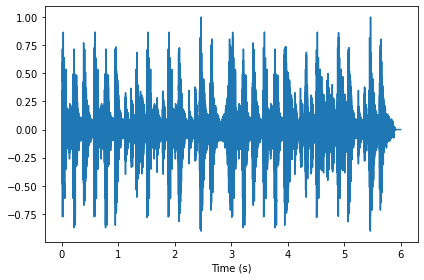
\includegraphics[width=0.75\textwidth]{samp1.png}
		\caption{Достаточно интересный сигнал}
		\label{fig:samp1}
	\end{figure}
	\begin{figure}[H]
		\centering
		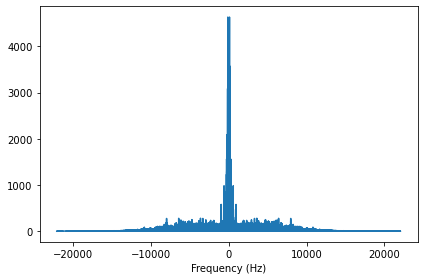
\includegraphics[width=0.75\textwidth]{samp2.png}
		\caption{Спектр этого сигнала}
		\label{fig:samp2}
	\end{figure}
	\begin{lstlisting}[language=Python,caption=Функция для выборки]
		from thinkdsp import Wave

		def sample(wave, factor):	
			ys = np.zeros(len(wave))
			ys[::factor] = wave.ys[::factor]
			return Wave(ys, framerate = wave.framerate)

		sampled = sample(wave, 4)
		sampled.make_spectrum(full = True).plot()
	\end{lstlisting}
	\begin{figure}[H]
		\centering
		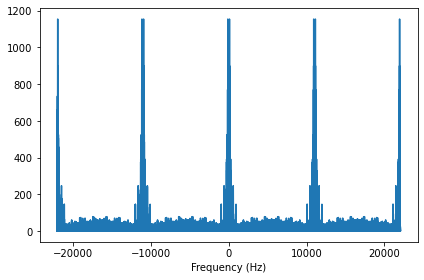
\includegraphics[width=0.75\textwidth]{samp3.png}
		\caption{Спектр сигнала после выборки}
		\label{fig:samp3}
	\end{figure}
	Результат звучит не очень хорошо, из-за дополнительных компонентов. Попробуем выяснить, откуда они появляются.
	\begin{lstlisting}[language=Python,caption=Функция для создания явных импульсов]
		def make_impulses(wave, factor):
			ys = np.zeros(len(wave))
			ys[::factor] = 1
			ts = np.arange(len(wave)) / wave.framerate
			return Wave(ys, ts, wave.framerate)

		impulses = make_impulses(wave, 4)
		sampled = wave * impulses
		impulses.make_spectrum(full = True).plot()
	\end{lstlisting}
	\begin{figure}[H]
		\centering
		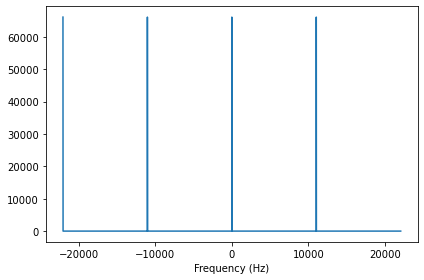
\includegraphics[width=0.75\textwidth]{samp4.png}
		\caption{Спектр сигнала после умножения на импульсы}
		\label{fig:samp4}
	\end{figure}
	Умножение на импульсы создает 4 сдвинутые копии исходного спектра. При умножении на пачку импульсов происходит свертка с ДПФ пачки импульсов.
	\begin{lstlisting}[language=Python,caption=Изменение количества импульсов]
		def show_impulses(wave, factor):
			impulses = make_impulses(wave, factor)
			plt.subplot(1, 2, 1)
			impulses.segment(0, 0.001).plot_vlines(linewidth=2)
			plt.subplot(1, 2, 2)
			impulses.make_spectrum(full = True).plot()

		slider = widgets.IntSlider(min=2, max=32, value=4)
		interact(show_impulses, wave = fixed(wave), factor = slider);
	\end{lstlisting}
	\begin{figure}[H]
		\centering
		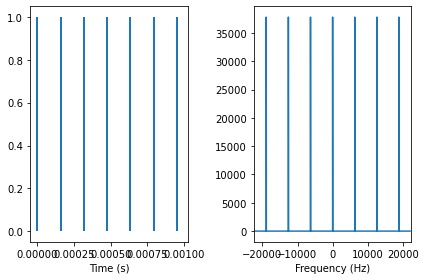
\includegraphics[width=1.0\textwidth]{samp5.png}
		\caption{Зависимость формы спектра от количества импульсов}
		\label{fig:samp5}
	\end{figure}
	Чем меньше количество импульсов, тем дальше они удаляются друг от друга во временной области и тем ближе копии спектра сближаются в частотной области.
	\begin{lstlisting}[language=Python,caption=Применим ФНЧ]
		spectrum = sampled.make_spectrum(full = True)
		spectrum.low_pass(5512.5)
		spectrum.plot()
		filtered = spectrum.make_wave()
	\end{lstlisting}
	\begin{figure}[H]
		\centering
		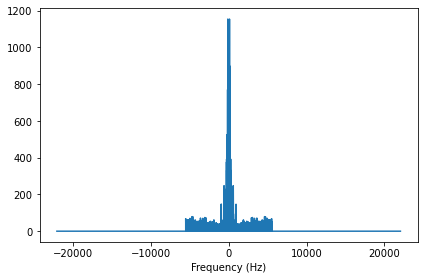
\includegraphics[width=0.75\textwidth]{samp6.png}
		\caption{Спектр после применения ФНЧ}
		\label{fig:samp6}
	\end{figure}
	Результат звучит совсем не так, как оригинал, из-за дополнительных копий в спектре.
	\begin{lstlisting}[language=Python,caption=Сравнение исходного и полученного сигнала]
		def plot_segments(original, filtered):
			start = 1
			duration = 0.01
			original.segment(start = start, duration = duration).plot(color = 'gray')
			filtered.segment(start = start, duration = duration).plot()

		plot_segments(wave, filtered)
	\end{lstlisting}
	\begin{figure}[H]
		\centering
		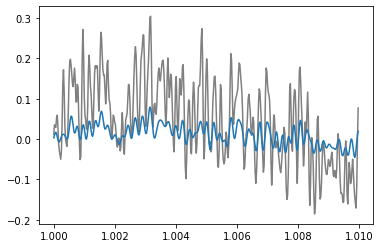
\includegraphics[width=0.75\textwidth]{samp7.png}
		\caption{Они явно не совпадают}
		\label{fig:samp7}
	\end{figure}
	\begin{lstlisting}[language=Python,caption=Возьмем другой сигнал]
		wave = read_wave('328878__tzurkan__guitar-phrase-tzu.wav')
		wave.normalize()
		wave.plot()
		wave.make_spectrum(full = True).plot()
	\end{lstlisting}
	\begin{figure}[H]
		\centering
		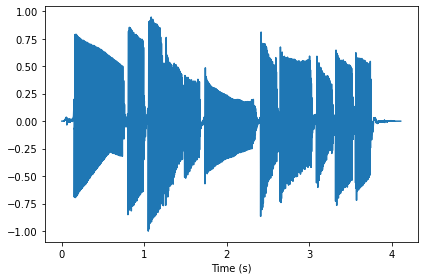
\includegraphics[width=0.75\textwidth]{samp8.png}
		\caption{Сигнал игры на бас-гитаре}
		\label{fig:samp8}
	\end{figure}
	\begin{figure}[H]
		\centering
		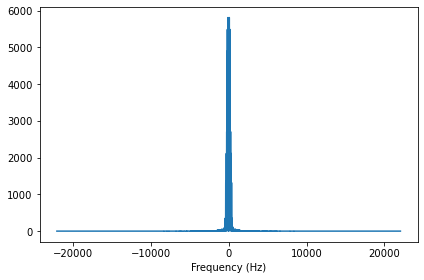
\includegraphics[width=0.75\textwidth]{samp9.png}
		\caption{Спектр этого сигнала}
		\label{fig:samp9}
	\end{figure}
	\begin{lstlisting}[language=Python,caption=Сделаем выборку сигнала]
		sampled = sample(wave, 4)
		sampled.make_spectrum(full = True).plot()
	\end{lstlisting}
	\begin{figure}[H]
		\centering
		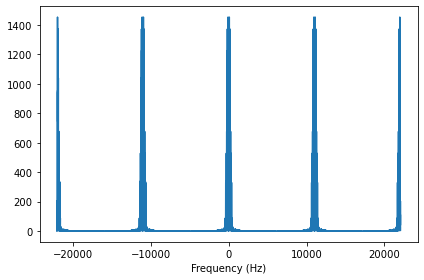
\includegraphics[width=0.75\textwidth]{samp10.png}
		\caption{Спектр сигнала после выборки}
		\label{fig:samp10}
	\end{figure}
	\begin{lstlisting}[language=Python,caption=Функция для построения прямоугольного фильтра]
		from thinkdsp import Spectrum

		def make_boxcar(spectrum, factor):
			fs = np.copy(spectrum.fs)
			hs = np.zeros_like(spectrum.hs)
			cutoff = (spectrum.framerate / 2) / factor
			for i, f in enumerate(fs):
				if abs(f) <= cutoff: hs[i] = 1
			return Spectrum(hs, fs, spectrum.framerate, full = spectrum.full)

		spectrum = sampled.make_spectrum(full = True)
		boxcar = make_boxcar(spectrum, 4)
		boxcar.plot()
	\end{lstlisting}
	\begin{figure}[H]
		\centering
		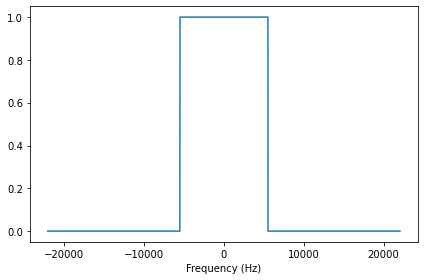
\includegraphics[width=0.75\textwidth]{samp11.png}
		\caption{Спектр прямоугольного фильтра}
		\label{fig:samp11}
	\end{figure}
	\begin{lstlisting}[language=Python,caption=Применим прямоугольный фильтр и результат сравним с исходным сигналом]
		filtered = (spectrum * boxcar).make_wave()
		filtered.scale(4)
		filtered.make_spectrum(full = True).plot()
		plot_segments(wave, filtered)
		diff = wave.ys - filtered.ys
		plt.plot(diff.real)
	\end{lstlisting}
	\begin{figure}[H]
		\centering
		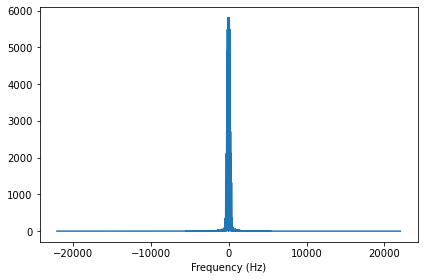
\includegraphics[width=0.75\textwidth]{samp12.png}
		\caption{Спектр отфильтрованного сигнала}
		\label{fig:samp12}
	\end{figure}
	\begin{figure}[H]
		\centering
		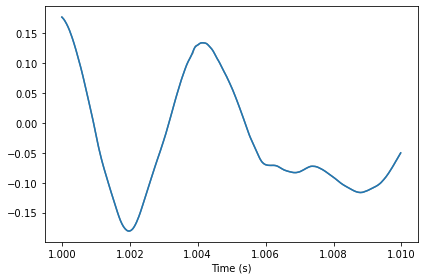
\includegraphics[width=0.75\textwidth]{samp13.png}
		\caption{Сегмент отфильтрованного сигнала}
		\label{fig:samp13}
	\end{figure}
	\begin{figure}[H]
		\centering
		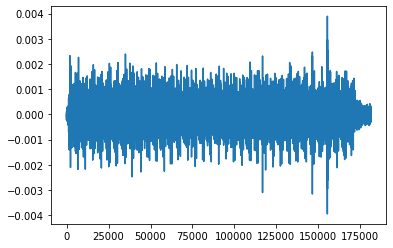
\includegraphics[width=0.75\textwidth]{samp14.png}
		\caption{Сравнение с исходным сигналом}
		\label{fig:samp14}
	\end{figure}
	Полученный сигнал не полностью идентичен исходному, потому что исходный сигнал имел некоторые компоненты на высоких частотах, но ими можно пренебречь.
	\begin{lstlisting}[language=Python,caption=Окно свертки]
		sinc = boxcar.make_wave()
		ys = np.roll(sinc.ys, 50)
		plt.plot(ys[:100].real)
	\end{lstlisting}
	\begin{figure}[H]
		\centering
		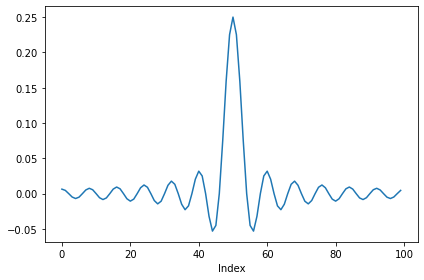
\includegraphics[width=0.75\textwidth]{samp15.png}
		\caption{Так выглядит окно свертки}
		\label{fig:samp15}
	\end{figure}

	\chapter{Интерполяция}
	Здесь мы узучаем \sloppy{\texttt{sinc}}-функцию.
	\begin{lstlisting}[language=Python,caption=Увеличим масштаб]
		start = 1.0
		duration = 0.01
		factor = 8
		short = wave.segment(start=start, duration=duration)
		short.plot()
		sampled = sample(short, factor)
		sampled.plot_vlines(color = 'gray')
	\end{lstlisting}
	\begin{figure}[H]
		\centering
		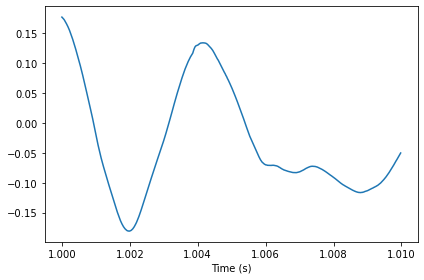
\includegraphics[width=0.75\textwidth]{sinc1.png}
		\caption{Уменьшенный сегмент сигнала}
		\label{fig:sinc1}
	\end{figure}
	\begin{figure}[H]
		\centering
		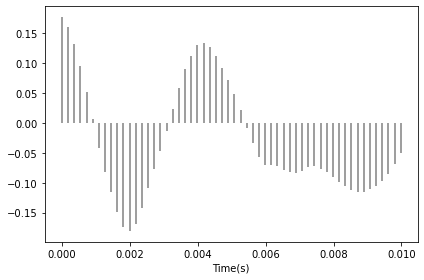
\includegraphics[width=0.75\textwidth]{sinc2.png}
		\caption{Выборки сигнала}
		\label{fig:sinc2}
	\end{figure}
	\begin{lstlisting}[language=Python,caption=Изменение положения sinc-функции]
		spectrum = sampled.make_spectrum()
		boxcar = make_boxcar(spectrum, factor)
		sinc = boxcar.make_wave()
		sinc.shift(sampled.ts[0])
		sinc.roll(len(sinc) // 2)
		sinc.plot()
	\end{lstlisting}
	\begin{figure}[H]
		\centering
		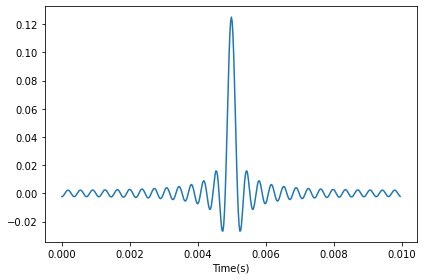
\includegraphics[width=0.75\textwidth]{sinc3.png}
		\caption{sinc-функция расположена посередине}
		\label{fig:sinc3}
	\end{figure}
	\begin{lstlisting}[language=Python,caption=Исследование sinc-функции]
		def plot_sinc_demo(wave, factor, start = None, duration = None):

			def make_sinc(t, i, y):
				sinc = boxcar.make_wave()
				sinc.shift(t)
				sinc.roll(i)
				sinc.scale(y * factor)
				return sinc
 
			def plot_sincs(wave):
				t0 = wave.ts[0]
				for i in range(0, len(wave), factor):
					sinc = make_sinc(t0, i, wave.ys[i])
					seg = sinc.segment(start, duration)
					seg.plot(color = 'green', linewidth = 0.5, alpha = 0.3)
					if i == 0: total = sinc
					else: total += sinc     
				seg = total.segment(start, duration)        
				seg.plot(color = 'blue', alpha = 0.5)

			sampled = sample(wave, factor)
			spectrum = sampled.make_spectrum()
			boxcar = make_boxcar(spectrum, factor)
			start = wave.start if start is None else start
			duration = wave.duration if duration is None else duration   
			sampled.segment(start, duration).plot_vlines(color = 'gray')
			wave.segment(start, duration).plot(color = 'gray')
			plot_sincs(wave)

		plot_sinc_demo(short, 4)
	\end{lstlisting}
	\begin{figure}[H]
		\centering
		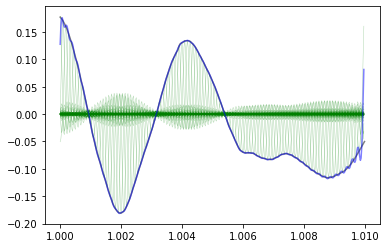
\includegraphics[width=0.75\textwidth]{sinc4.png}
		\caption{Результат исследования работы sinc-функции}
		\label{fig:sinc4}
	\end{figure}
	Тонкие зеленые линии - это сдвинутые, масштабированные копии  sinc-функции. Синяя линия - это сумма sinc-функций. Серая линия - это исходная функция. Сумма \sloppy{\texttt{sinc}}-функций интерполируется между образцами и восстанавливает исходную волну.
	\begin{lstlisting}[language=Python,caption=Рассмотрим результат внимательнее]
		start = short.start + 0.004
		duration = 0.00061
		plot_sinc_demo(short, 4, start, duration)
		decorate(xlim = [start, (start + duration)], ylim = [-0.05, 0.17])
	\end{lstlisting}
	\begin{figure}[H]
		\centering
		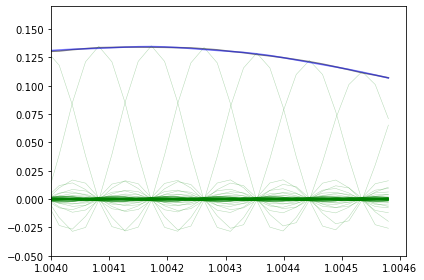
\includegraphics[width=0.75\textwidth]{sinc5.png}
		\caption{Крупный план}
		\label{fig:sinc5}
	\end{figure}
	Вертикальные серые линии - это выборки. Тонкие зеленые линии - это сдвинутые, масштабированные копии \sloppy{\texttt{sinc}}-функции. В этом сегменте интерполяция очень хорошо соответствует исходной волне. Сумма \sloppy{\texttt{sinc}}-функций идентична оригинальному сигналу.
	
	\chapter{Упражнения}
	\section{Задание 3}
	Фильтрация частоты до выборки - фильтр сглаживания.
	\begin{lstlisting}[language=Python,caption=Соло на барабане]
		wave = read_wave('263868__kevcio__amen-break-a-160-bpm.wav')
		wave.normalize()
		wave.plot()
		spectrum = wave.make_spectrum(full = True)
		spectrum.plot()
	\end{lstlisting}
	\begin{figure}[H]
		\centering
		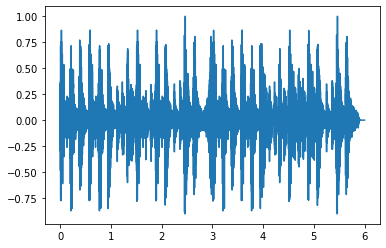
\includegraphics[width=0.75\textwidth]{task1.png}
		\caption{График сигнала}
		\label{fig:task1}
	\end{figure}
	\begin{figure}[H]
		\centering
		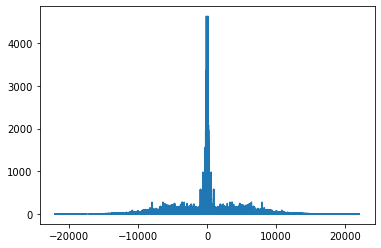
\includegraphics[width=0.75\textwidth]{task2.png}
		\caption{И его спектр}
		\label{fig:task2}
	\end{figure}
	\begin{lstlisting}[language=Python,caption=Фильтр сглаживания]
		framerate = wave.framerate / 5
		cutoff = framerate / 2 - 1
		spectrum.low_pass(cutoff)
		spectrum.plot()
	\end{lstlisting}
	\begin{figure}[H]
		\centering
		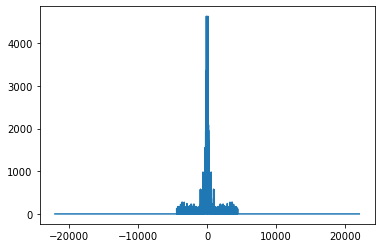
\includegraphics[width=0.75\textwidth]{task3.png}
		\caption{Результат работы фильтра}
		\label{fig:task3}
	\end{figure}
	После фильтрации сигнал все еще довольно хорошо звучит.
	\begin{lstlisting}[language=Python,caption=Выборка]
		filtered = spectrum.make_wave()
		sampled = sample(filtered, 5)
		sampled_spectrum = sampled.make_spectrum(full = True)
		sampled_spectrum.plot()
	\end{lstlisting}
	\begin{figure}[H]
		\centering
		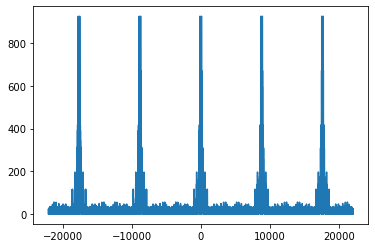
\includegraphics[width=1.0\textwidth]{task4.png}
		\caption{Спектр сигнала после выборки}
		\label{fig:task4}
	\end{figure}
	\begin{lstlisting}[language=Python,caption=Строим спектр полученного сигнала]
		sampled_spectrum.low_pass(cutoff)
		sampled_spectrum.plot()
		sampled_spectrum.scale(5)
		spectrum.plot()
		sampled_spectrum.plot()
	\end{lstlisting}
	\begin{figure}[H]
		\centering
		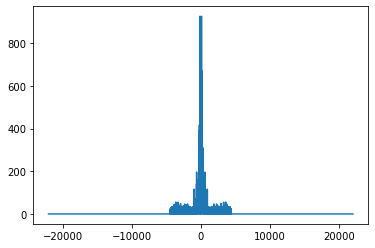
\includegraphics[width=0.75\textwidth]{task5.png}
		\caption{Спектр полученного сигнала}
		\label{fig:task5}
	\end{figure}
	\begin{figure}[H]
		\centering
		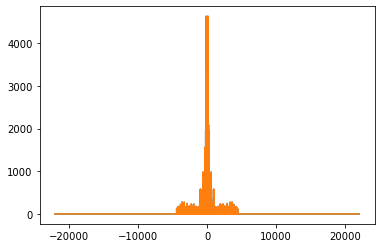
\includegraphics[width=0.75\textwidth]{task6.png}
		\caption{Сравнение полученного спектра с исходным спектром}
		\label{fig:task6}
	\end{figure}
	Разница между ними близка к 0.
	\begin{lstlisting}[language=Python,caption=Разница между интерполяцией и фильтрацией сигнала]
		interpolated = sampled_spectrum.make_wave()
		filtered.plot()
		interpolated.plot()
	\end{lstlisting}
	\begin{figure}[H]
		\centering
		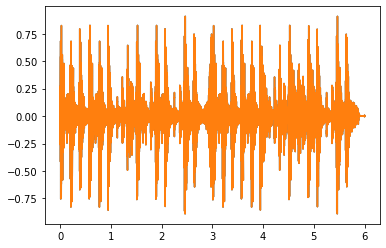
\includegraphics[width=0.75\textwidth]{task7.png}
		\caption{Разница почти равняется нулю}
		\label{fig:task7}
	\end{figure}

	\chapter{Вывод}
	В данной работе мы познакомились с работой ампдитудной модуляции, узнали, как влияет количество выборок на качество сигнала, и немного изучили алгоритм \sloppy{\texttt{sinc}}-функции.
\end{document}